\section{Introduktion til Occupancy Grid}
Til at kortlægge rummet robotten befinder sig i er der valgt at bruge \textit{occupancy grid}.
Teorien bag denne algoritme vil blive beskrevet i dette afsnit

\subsection{Overblik}
Den overordnede idé bag et occupancy grid er at lave en ensartet inddeling af sit kort, hvor hver enkelt celle er repræsenteret af en binær tilfældig variabel der fortæller om den pågældende celle er 'optaget' eller ej, hvor optaget betegnes som sandsynligheden $\mathcal{P}(occupied) = 1$.
Til at begynde med initialiseres hver enkelt celle med værdien $\mathcal{P}(occupied) = 0,5$ som en indikation på den aktuelle tilstand endnu ikke er kendt.
En 'ledig' celle har således værdien $\mathcal{P}(occupied) = 0$.

En simpel illustration af et occupancy grid map for det kørselsmiljø der er opstillet for vores robot kan ses på \cref{map:approx_occupancy_grid}.

\begin{figure}[h] % Kørselsmiljø og et occupancy grid
\centering
	\begin{subfigure}[b]{.45\textwidth}
	\centering
	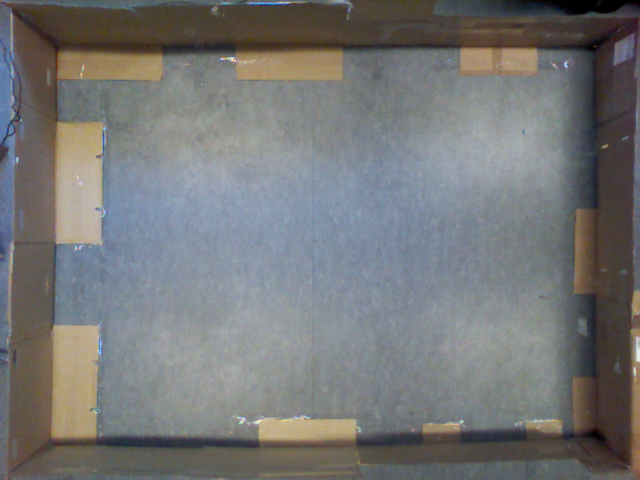
\includegraphics[width=\textwidth]{verden/oppefra}
	\caption{Aktuelt Kørselsmiljø}
	\label{map:world}
	\end{subfigure}
	\begin{subfigure}[b]{.45\textwidth}
	\centering
	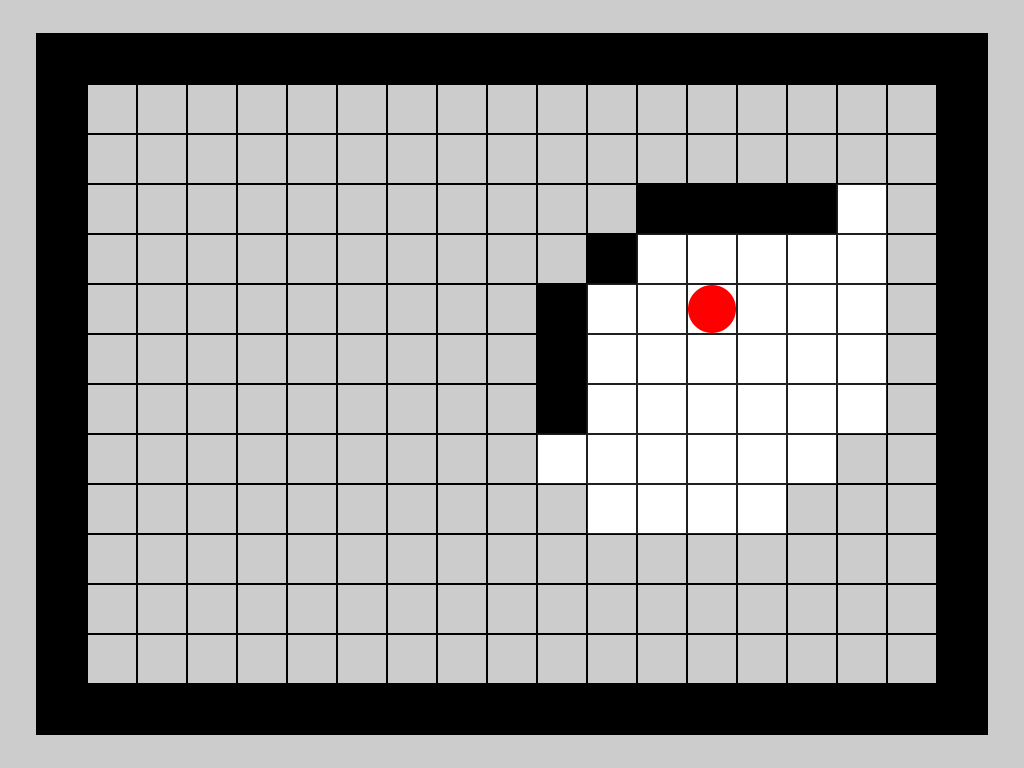
\includegraphics[width=\textwidth]{verden/occupancy_grid_verden}
	\caption{Eksempel på Occupancy Grid}
	\label{map:occupancy_grid}
	\end{subfigure}
\caption{Illustration af et occupancy grid baseret på projekts kørselsmiljø for robotten. Sorte celler i \cref{map:occupancy_grid} indikerer at $\mathcal{P}(occupied) = 1$, hvilket betegner væggene i kørselsmiljøet (\cref{map:world}). Hvide celler indikerer at $\mathcal{P}(occupied) = 0$ og grå celler angiver ikke-udforsket område. Den røde cirkel indikerer robottens position.}
\label{map:approx_occupancy_grid}
\end{figure}

\subsection{Vertikal og horisontal sensor model}
\stefan{kildehenvisning}
Hvis vi antager, at alle objekter i opstillingen er placeret vinkelret til områdets x og y akser,
kan vi konstruere en forholdsvis simpel basal sensormodel.
Først beregner vi afstanden fra robotten til den pågældende celle i vores occupancy grid.

\begin{equation}
r_{actual} = \mid x_{cell} - x_{robot} + y_{cell} - y_{robot} \mid
\end{equation}

Sandsynligheden for at cellen er  \emph{occupied} tildeles således.

\begin{equation}
\begin{split}
l_{res} = \begin{cases} 
	l_0 &\text{hvis }r_{actual} > \text{min}(z_{max},z_t+\frac{\alpha}{2}) \\ 
	l_{occ} &\text{hvis } z_t-\frac{\alpha}{2} \leq r_{actual} \leq z_t+\frac{\alpha}{2}\\ 
	l_{free} &\text{ellers}  
\end{cases}
\end{split}
\end{equation}

Hvor værdien $\alpha$ er den gennemsnitlige dybde af et objekt i området.
Modellen vil se således ud beskrevet i pseudokode:

\begin{algorithm}[H]
\textbf{InversSensorModel($i, x_t, z_t$)} \\
Let $x_i,y_i$ be the center-of-mass of $m_i$ \\
$r = |x_i - x + y_i - y|$ \\
\If{$r > min(z_{max}, z_t + \frac{\alpha}{2}$)}{
	\Return{$l_0$}
}
\ElseIf{$z_t - \frac{\alpha}{2} \le r \le z + \frac{\alpha}{2}$}{
	\Return{$l_{occ}$}
}
\Else{
	\Return{$l_{free}$}
}
\caption{Invers sensor model algoritme}
\label{alg:inversesensormodel}
\end{algorithm}

\subsubsection{Gaussisk sensor model}

% forklaring af gaussisk støj (central limit theorem)
% tilfældige fejl vil tilnærme sig en gausssisk kurve.
I modellen beskrevet i det forgående afsnit, antog vi at en celle
med afstanden $\frac{\alpha}{2}$ fra robottens måling på $z_t$ havde
samme sandsynlighed som en celle med afstanden 0 fra $z_t$.

Hvis vi antager, at de celler som ligger tættere på robottens måling,
har en større sandsynlighed for at være \emph{occupied}. 
Så kan vi konstruere en sensor model med en glidende overgang fra værdien $l_{occ}$ for 
cellen i $z_t$ til værdien $l_{free}$ for cellen på positionen $z_t \pm \frac{\alpha}{2}$. 

Da summen af uafhængige fejlmålinger, ifølge \emph{central limit theorem} vil tilnærme sig
den gaussiske normalfordeling. \cite[p. 223]{ArtificialIntelligence}
Vil det være en god approximation for robottens måleusikkerhed.


Vi kan anvende en passende normalfordeling $\mathcal{N}(z_t,\big(\frac{\alpha}{6}\big)^2)$ 




\begin{equation}
\mathcal{N}\bigg(z_t,\bigg(\frac{\alpha}{6}\bigg)^2\bigg) = 
\frac{1}{\sqrt{2 \pi \big(\frac{\alpha}{6}\big)^2}}e^{- \frac{(x - z_t)^2}{2 (\frac{\alpha}{6})^2}}
\end{equation}

Den nye tildeling af sandsynlighed til cellen vil nu se således ud.

\begin{equation}
l_{res} = \begin{cases} 
	l_0 &\text{hvis }r_{actual} > \text{min}(z_{max},z_t+\frac{\alpha}{2}) \\ 
	
	
	\eta \int_{r-\rho}^{r+\rho} \frac{1}{\sqrt{2 \pi \big(\frac{\alpha}{6}\big)^2}}e^{- \frac{(r_{actual} - z_t)^2}{2 (\frac{\alpha}{6})^2}}\, \mathrm{d}r
		&\text{hvis } z_t-\frac{\alpha}{2} \leq r_{actual} \leq z_t+\frac{\alpha}{2}\\ 

	l_{free} &\text{ellers}	
\end{cases}
\end{equation}
\\
Hvor $\rho$ er en passende konstant og $\eta$ er en normaliseringskonstant.



\thilemann{Mangler der noget her?}



%
%\subsection{Generel udgave af sensor modellen}
%
%% objekter kan placeres i alle vinkler
%
%\subsubsection{Generel model med gaussisk støj}
%
%% gaussisk støj i 2-d
%
%
%\subsection{tilpasset sensor model}
%
%
%% overfitting
%
%\subsection{sensor model baseret på målinger}
%
%% fejl i sensor er ikke nødvendigvis 'tilfældige' eller uafhængige
%% en generel sensormodel som benytter en sandsynlighedsdistribution som vi selv har målt.
%
%
%\subsection{data udledet udfra robottens placering}
%
%% forbedring hvor vi tager højde for robotten
%
%
%\section{Forward Sensor Model	}
%
%
%














\
